% Options for packages loaded elsewhere
\PassOptionsToPackage{unicode}{hyperref}
\PassOptionsToPackage{hyphens}{url}
%
\documentclass[
]{book}
\usepackage{lmodern}
\usepackage{amssymb,amsmath}
\usepackage{ifxetex,ifluatex}
\ifnum 0\ifxetex 1\fi\ifluatex 1\fi=0 % if pdftex
  \usepackage[T1]{fontenc}
  \usepackage[utf8]{inputenc}
  \usepackage{textcomp} % provide euro and other symbols
\else % if luatex or xetex
  \usepackage{unicode-math}
  \defaultfontfeatures{Scale=MatchLowercase}
  \defaultfontfeatures[\rmfamily]{Ligatures=TeX,Scale=1}
\fi
% Use upquote if available, for straight quotes in verbatim environments
\IfFileExists{upquote.sty}{\usepackage{upquote}}{}
\IfFileExists{microtype.sty}{% use microtype if available
  \usepackage[]{microtype}
  \UseMicrotypeSet[protrusion]{basicmath} % disable protrusion for tt fonts
}{}
\makeatletter
\@ifundefined{KOMAClassName}{% if non-KOMA class
  \IfFileExists{parskip.sty}{%
    \usepackage{parskip}
  }{% else
    \setlength{\parindent}{0pt}
    \setlength{\parskip}{6pt plus 2pt minus 1pt}}
}{% if KOMA class
  \KOMAoptions{parskip=half}}
\makeatother
\usepackage{xcolor}
\IfFileExists{xurl.sty}{\usepackage{xurl}}{} % add URL line breaks if available
\IfFileExists{bookmark.sty}{\usepackage{bookmark}}{\usepackage{hyperref}}
\hypersetup{
  pdftitle={Micro and Macro Data},
  pdfauthor={Mauritz van den Worm},
  hidelinks,
  pdfcreator={LaTeX via pandoc}}
\urlstyle{same} % disable monospaced font for URLs
\usepackage{longtable,booktabs}
% Correct order of tables after \paragraph or \subparagraph
\usepackage{etoolbox}
\makeatletter
\patchcmd\longtable{\par}{\if@noskipsec\mbox{}\fi\par}{}{}
\makeatother
% Allow footnotes in longtable head/foot
\IfFileExists{footnotehyper.sty}{\usepackage{footnotehyper}}{\usepackage{footnote}}
\makesavenoteenv{longtable}
\usepackage{graphicx,grffile}
\makeatletter
\def\maxwidth{\ifdim\Gin@nat@width>\linewidth\linewidth\else\Gin@nat@width\fi}
\def\maxheight{\ifdim\Gin@nat@height>\textheight\textheight\else\Gin@nat@height\fi}
\makeatother
% Scale images if necessary, so that they will not overflow the page
% margins by default, and it is still possible to overwrite the defaults
% using explicit options in \includegraphics[width, height, ...]{}
\setkeys{Gin}{width=\maxwidth,height=\maxheight,keepaspectratio}
% Set default figure placement to htbp
\makeatletter
\def\fps@figure{htbp}
\makeatother
\setlength{\emergencystretch}{3em} % prevent overfull lines
\providecommand{\tightlist}{%
  \setlength{\itemsep}{0pt}\setlength{\parskip}{0pt}}
\setcounter{secnumdepth}{5}
\usepackage{booktabs}
\usepackage[]{natbib}
\bibliographystyle{apalike}

\title{Micro and Macro Data}
\author{Mauritz van den Worm}
\date{2020-09-29}

\begin{document}
\maketitle

{
\setcounter{tocdepth}{1}
\tableofcontents
}
\hypertarget{intro}{%
\chapter{Introduction}\label{intro}}

In this write-up we explore the role macro-economic data plays on the dynamics of calendar spreads. This is done by comparing the affects of macro- to micro-economic data on calendar spreads. The size of the effects are measured in two ways

\begin{itemize}
\tightlist
\item
  Feature Importance using

  \begin{itemize}
  \tightlist
  \item
    MDI - Mean Decrease Impurity
  \item
    MDA - Mean Decrease Accuracy
  \item
    SFI - Single Feature Importance
  \item
    CFI - Clustered Feature Importance
  \item
    SHAP - Shapley Feature Importance
  \item
    PCA - Principle Component Analysis
  \item
    For details on the above methods see Advances in Financial Machine Learning
  \end{itemize}
\item
  Fingerprint method of Yimou Li, David Turkington and Alireza Yazdani
\end{itemize}

The macro-economic features we consider are

\begin{itemize}
\tightlist
\item
  The mean price of the near dated WTI crude ontract during the previous month
\item
  Dollar Index
\item
  Rubble vs USD exachange rate
\item
  Libor
\end{itemize}

The micro-economic features we consider are made up of the stock-to-usage numbers of the commodities considered in

\begin{itemize}
\tightlist
\item
  Argentina
\item
  Brazil
\item
  China
\item
  European Union
\item
  Russia
\item
  Ukraine
\item
  United States
\item
  World
\item
  World without China
\end{itemize}

\hypertarget{calendar-spreads}{%
\chapter{Calendar Spreads}\label{calendar-spreads}}

\hypertarget{introduction}{%
\section{Introduction}\label{introduction}}

One of our main flavours of relative value commodity alpha we like to harvest is to express our views using calendar spreads. This is where we take opposing views on different parts of the futures curve of a single commodity. This can be done in two ways

\begin{itemize}
\tightlist
\item
  Bull spreads: long the near dated and short the far dated contract
\item
  Bear Spreads : long the far dated and short the near dated
\end{itemize}

\hypertarget{curve-shapes}{%
\section{Curve Shapes}\label{curve-shapes}}

There are two basic futures curve shapes

\begin{itemize}
\item
  Contango
  When the near dated contracts are trading at a discount compared to the far dated contracts
\item
  Backwardation
  When the near dated contracts are trading at a premium compared to the far dated contracts
\end{itemize}

In the plots below we show example of what each case look like. On the y-axis we show the price of each of the contracts. The x-axis shows the expiration dates associated with each of the contracts. The codes at each point represent the standard market codes for the different maturities.

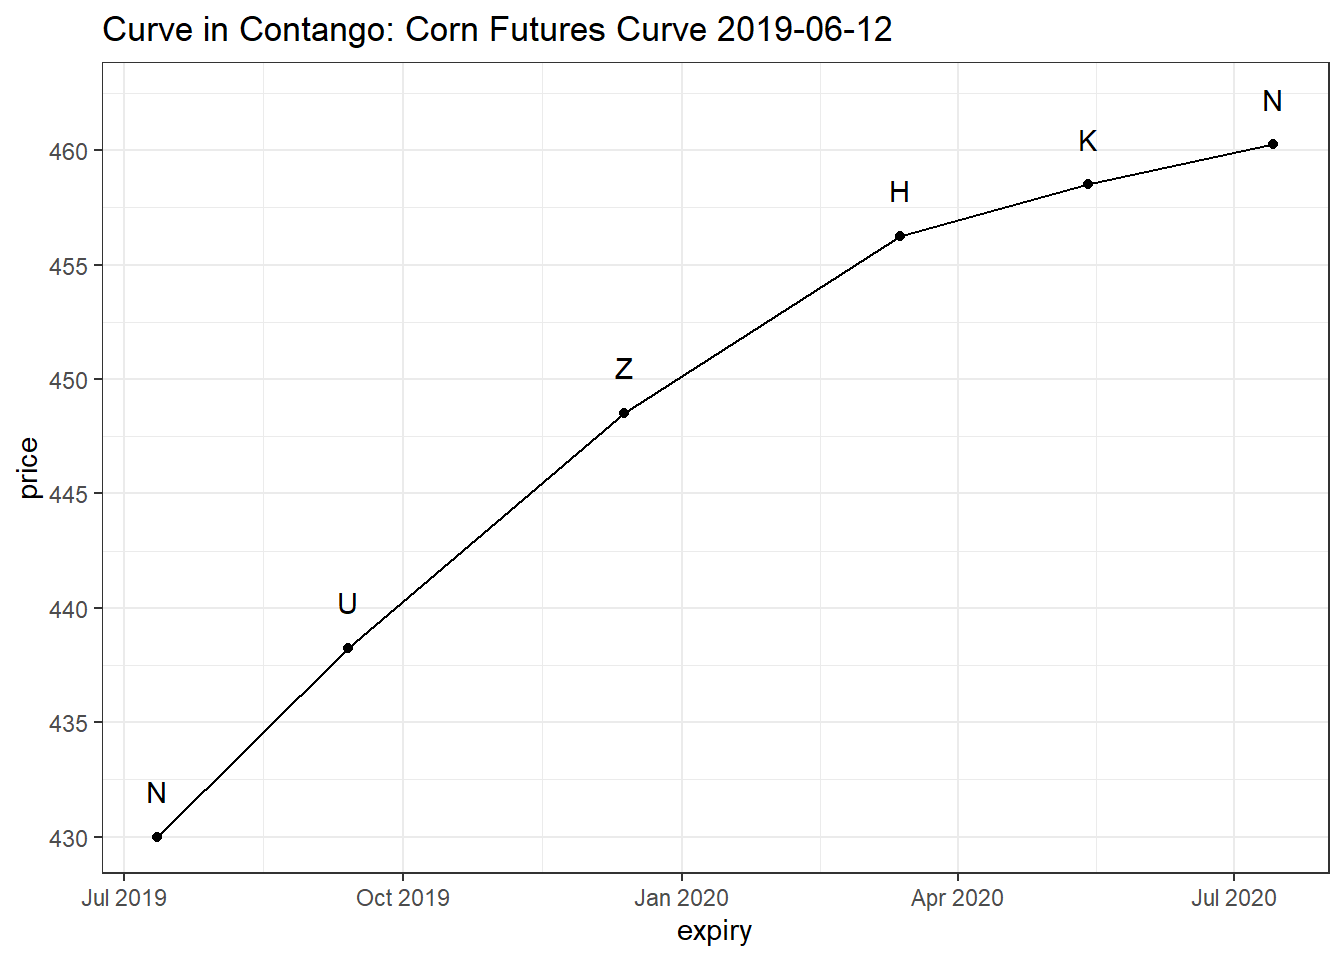
\includegraphics{calendar-spreads-macro-data_files/figure-latex/contango_plot-1.pdf}

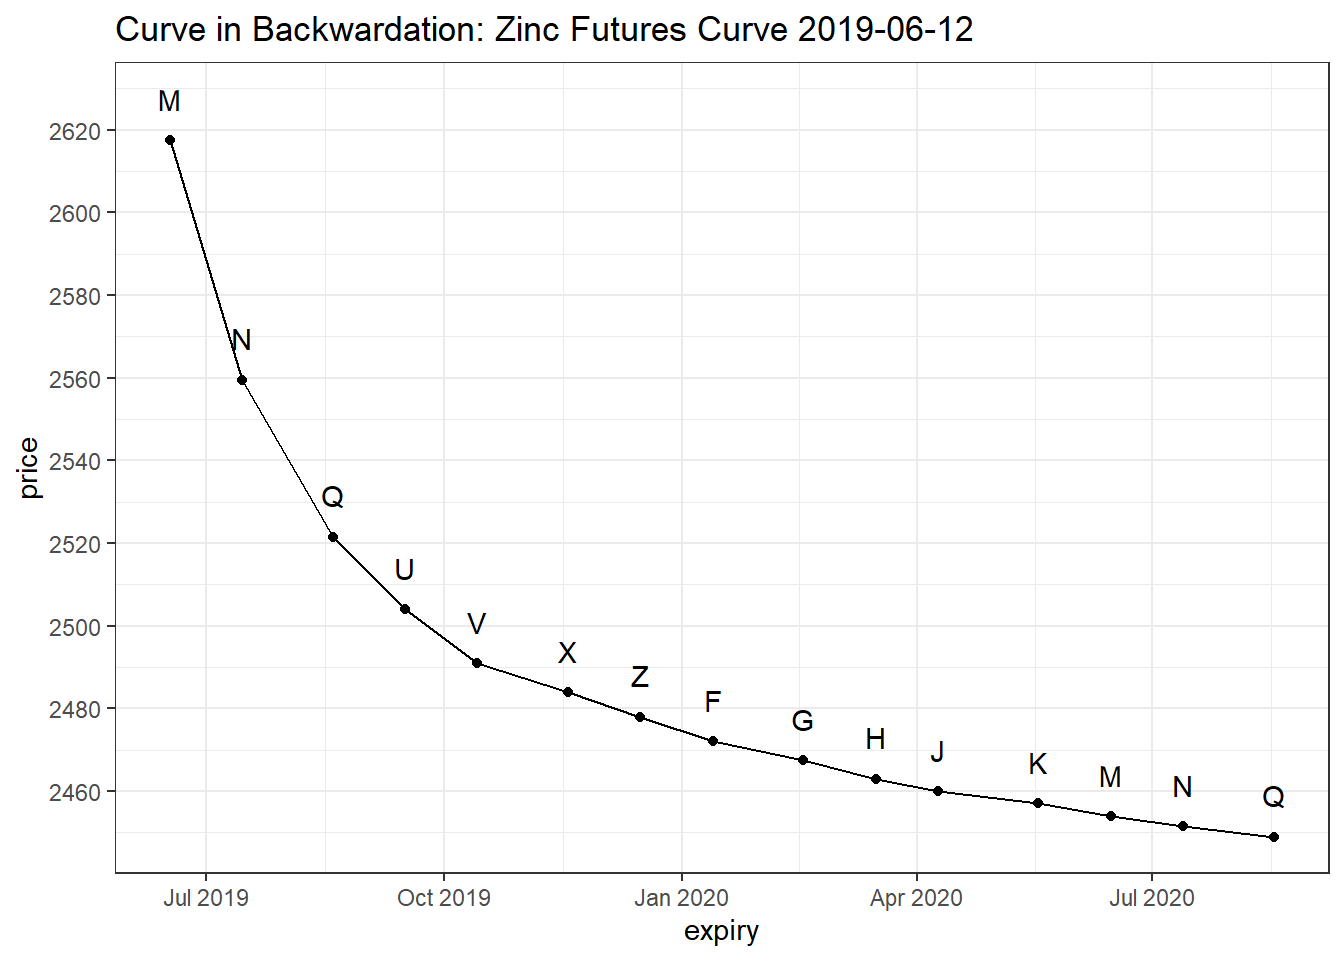
\includegraphics{calendar-spreads-macro-data_files/figure-latex/backwardation_plot-1.pdf}

Commodity futures curves are divided by obstacles to intertemporal arbitrage. The costlier the storage, the greater is the division and the variability of calendar spread moves. The segmented commodity futures curve is shaped by four factors:

\begin{itemize}
\tightlist
\item
  Funding and storage costs,
\item
  Expected supply and demand imbalanced,
\item
  Convenience yields and
\item
  Hedging pressure.
\end{itemize}

Under normal conditions commodity producers take short futures positions in the deferred parts fo the commodity futures curve in order to hedge against price drops. The investor or speculator that offers this insurance is paid a premium and takes a long position in the futures contract. This positive premium comes in the form of the carry premium. On the other hand, commodity consumers take long futures positions in nearer dated contracts in order to hedge against unexpected future price surges. The investor or speculator that offers this insurance receives a premium for taking up the risk and takes a short position, in which case contango arises.

When commodity stocks are in abundance the funding and storage costs can become high which forces the futures curve more contango. There is a maximum degree of contango the futures curve can have, given by full carry. The level of full carry depends on interest rates. For this reason we include Libor rates as part of our macro-economic indicators.

\hypertarget{notation}{%
\section{Notation}\label{notation}}

We define the value of a calendar spread as

\[
S_{ij} = P_i - P_j, \text{with } j > i.
\]
Here \(P_i\) and \(P_j\) represent the prices of contracts \(i\) and \(j\) respectively. Moreover, contract \(j\) expires after contract \(i\). In words, calendar spreads are calculated as the difference between the near and far dated futures contracts. A negative spread implies the near dated contract is trading at a discount compared to the far dated contract, i.e.~contango. Similarly, a positive spread implies that the near dated contract is trading at a premium with respect to the far dated contract, i.e.~backwardation.

\hypertarget{example}{%
\section{Example}\label{example}}

Below we consider an example of the Corn ZZ, or December-December calendar spread. On the y-axis we show the value of the spread and on the x-axis the stacked date. Note that the actual values of the years make no difference here. The point is to visualise the seasonal pattern that emerges.

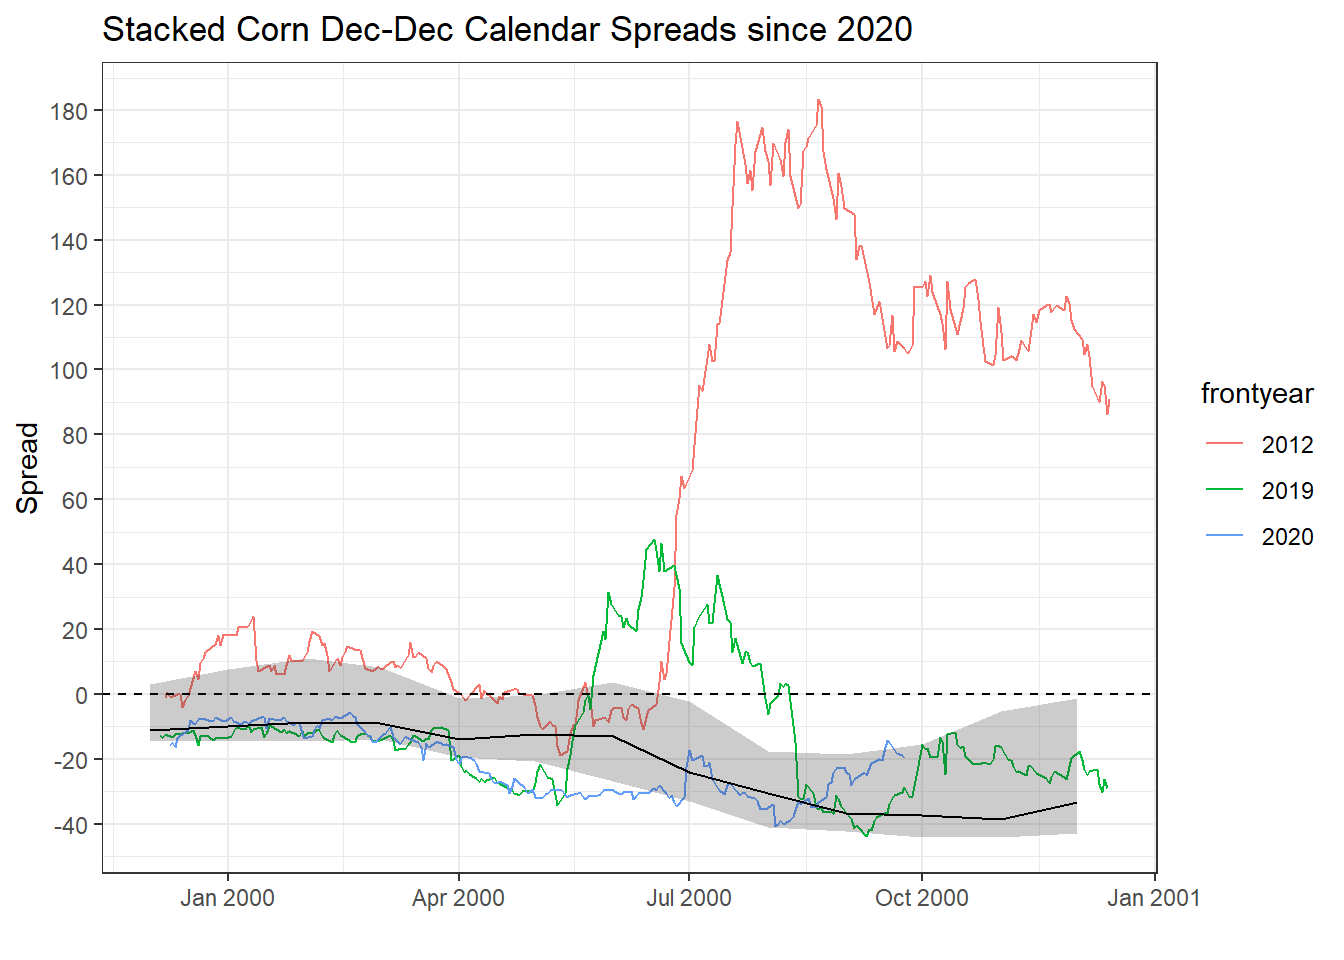
\includegraphics{calendar-spreads-macro-data_files/figure-latex/stacked_calendar_plot-1.pdf}

We highlight three years. The first is 2012, here shown in red. This year saw a massive drought in the United States which destroyed the production and forced the curve into a severe backwardation. The green curve shows how the spread evolved during 2019 and the blue curve represents the current spread. The solid black line represents the monthly median while the shaded region shows the 25th to 75th percentile. Half of the historical data lies within the shaded region. The horizontal dashed line is there to help distinguish between backwardation (\(S > 0\)) and contango (\(S < 0\)).

\hypertarget{different-calendar-spread-combinations}{%
\section{Different Calendar Spread Combinations}\label{different-calendar-spread-combinations}}

The Corn futures market has five different codes within each year

\begin{itemize}
\tightlist
\item
  H
\item
  K
\item
  N
\item
  U
\item
  Z
\end{itemize}

This implies that that are 25 different calendar spread combinations we can create using only the corn futures market. The table below shows all the different calendar combinations we can create.

H

K

N

U

Z

H

HH

HK

HN

HU

HZ

K

KH

KK

KN

KU

KZ

N

NH

NK

NN

NU

NZ

U

UH

UK

UN

UU

UZ

Z

ZH

ZK

ZN

ZU

ZZ

The table above highlights the extent of the different instruments available to trade when we want to express a view on Corn. The same applies to all the other commodities we cover.

\hypertarget{feature-importance}{%
\chapter{Feature Importance}\label{feature-importance}}

The study of feature importance is important in the modeling process and helps to find those features that have the greatest influence in predicting the chosen observable. In practice we make use of a collection of different feature importance techniques

\begin{itemize}
\tightlist
\item
  MDI - Mean Decrease Impurity
\item
  MDA - Mean Decrease Accuracy
\item
  SFI - Single Feature Importance
\item
  CFI - Clustered Feature Importance
\item
  SHAP - Shapley Feature Importance
\item
  PCA - Principle Component Analysis
\end{itemize}

To find the technique that overlaps with most with what we expect to see from a PCA we make use of the weighted tau technique.

\hypertarget{ml-model-performance}{%
\section{ML model performance}\label{ml-model-performance}}

In order to apply the methods outlined above we need to apply some machine learning techniques. Specifically, we apply two linear

\begin{itemize}
\tightlist
\item
  Multi-variate linear regression
\item
  Multi-variate lasso regression
\end{itemize}

and one non-linear algorithm

\begin{itemize}
\tightlist
\item
  Random Forest
\end{itemize}

The reason for apply these methods is twofold. The complicated relationships between different features in the context of financial problems does not have to be of a linear nature as is assumed in the majority of econometric literature. The second is that interaction effects between different features have historically been ignored.

Keeping with the Corn December-December data of before we show in the table below the model results of the three methods. The value is each of the cells is R-squared, the greater the number the better. We show the results of the model fit, i.e.~the in sample results, and also the model fit on data left out of the training sample. The out of sample results for the Random Forest model is considerably better than the two linear models.

Model

In Sample Score

Out of Sample Score

Random Forest

0.914

0.714

Linear Regression

0.464

0.278

Lasso Regression

0.460

0.292

The table below shows the best out of sample performance for each of the different calendar spread combinations. It is only in the case of the UU calendar spread that the lasso model outperformed the Random Forest model.

Calendar Reference

Model

In Sample Score

Out of Sample Score

HH

Random Forest

0.871

0.546

HK

Random Forest

0.866

0.590

HN

Random Forest

0.878

0.580

HU

Random Forest

0.937

0.751

HZ

Random Forest

0.947

0.737

KH

Random Forest

0.967

0.836

KK

Random Forest

0.958

0.866

KN

Random Forest

0.931

0.448

KU

Random Forest

0.965

0.817

KZ

Random Forest

0.969

0.840

NH

Random Forest

0.973

0.964

NK

Random Forest

0.967

0.936

NN

Random Forest

0.965

0.958

NU

Random Forest

0.970

0.879

NZ

Random Forest

0.968

0.965

UH

Random Forest

0.986

0.786

UK

Random Forest

0.984

0.751

UN

Random Forest

0.981

0.733

UU

Lasso Regression

0.799

0.656

UZ

Random Forest

0.989

0.813

ZH

Random Forest

0.784

0.399

ZK

Random Forest

0.883

0.471

ZN

Random Forest

0.841

0.433

ZU

Random Forest

0.891

0.477

ZZ

Random Forest

0.914

0.714

In the following we study the main contributing features of the best models shown in the table above.

\hypertarget{relevant-features}{%
\section{Relevant Features}\label{relevant-features}}

The plot below continues with the Corn December-December spread and shows the feature importance results in a bar chart. The y-axis labels the different features and the x-axis shows the value of feature importance. Here we can see that the \emph{daysdiff} feature, measuring the number of days until the expiry of the front dated contract plays a large role in the model performance. This might signify that the spread has strong seasonal behaviour, which we can confirm from the earlier plot showing the stacked calendar spread evolution. Other than the strong seasonality we can see that the value of the Rubble also plays a stong role. The value of crude oil and the libor rate doesn't seem to be predictive.

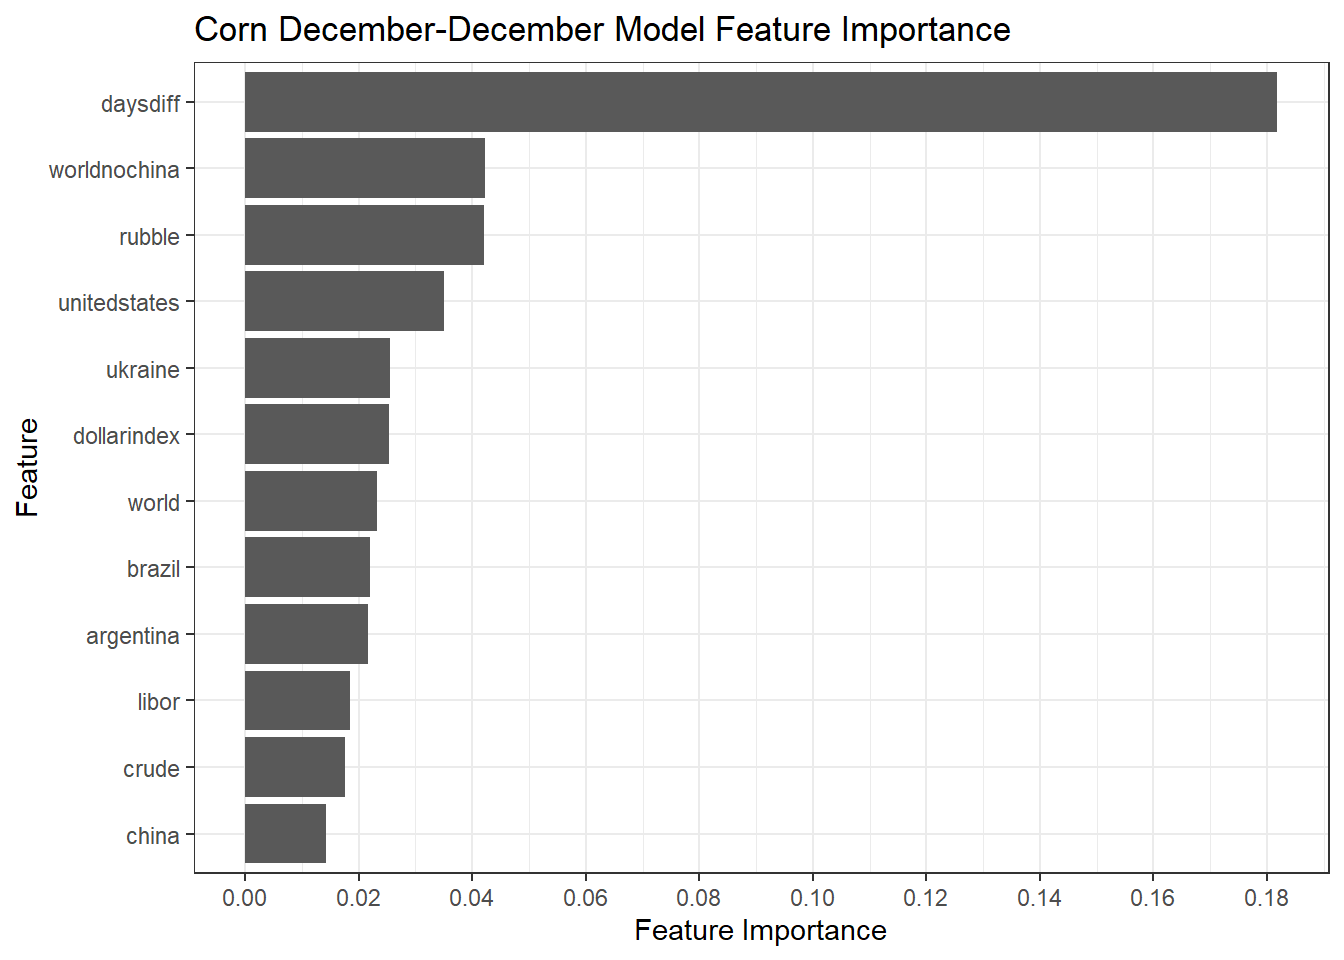
\includegraphics{calendar-spreads-macro-data_files/figure-latex/zz_fi_plot-1.pdf}

The plot below is similar to the one above, but this time we show the feature importance results for the Corn July-December spread, which was the best out of sample performing model. Here there seems to be much less of a seasonal behaviour compared to the December-December spread. Macro factors that influes this spread include the Dollar Index as well as the price of crude oil.

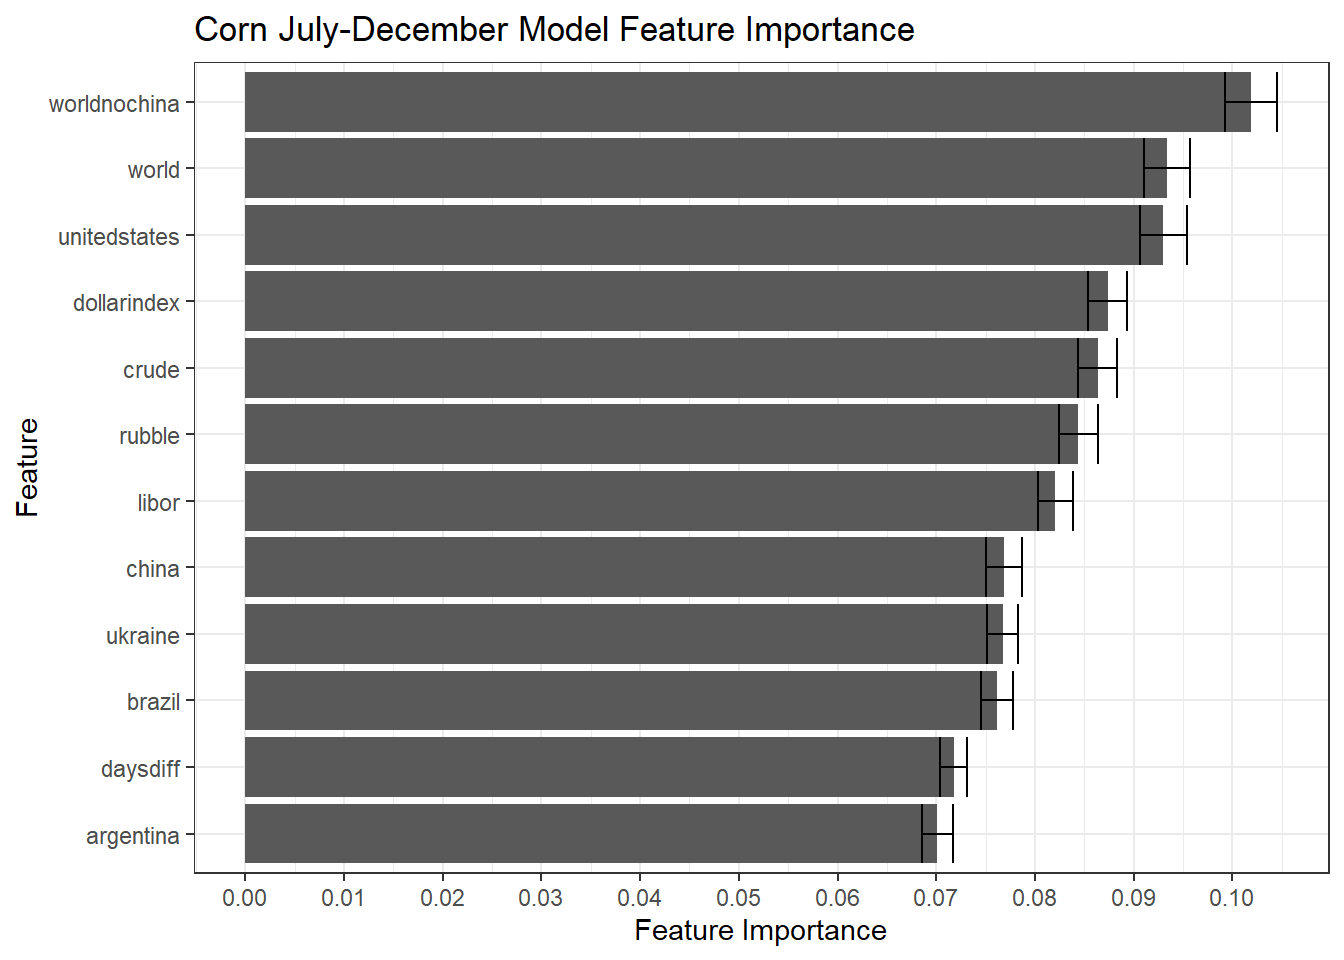
\includegraphics{calendar-spreads-macro-data_files/figure-latex/nz_fi_plot-1.pdf}

The table below aggregates the ranks of each of the features for every corn calendar spread. The smaller the number the more importance it carries in determining the future value of the spread.

feature

rank

worldnochina

1.92

daysdiff

3.16

unitedstates

3.80

world

4.64

rubble

5.24

ukraine

5.68

crude

6.04

dollarindex

6.48

libor

6.80

china

7.00

brazil

7.76

argentina

7.80

The table above shows that global corn stock-to-usage numbers without taking China into account seems to have the best predictive power followed by the days to expiry of the front month contract and United States corn stock-to-usage numbers. Here the value of the Dollar and the Libor rate seem to play more of a back seat role.

\hypertarget{fingerprint-method}{%
\chapter{Fingerprint Method}\label{fingerprint-method}}

\hypertarget{quick-overview-of-the-fingerprint-method}{%
\section{Quick Overview of the Fingerprint method}\label{quick-overview-of-the-fingerprint-method}}

This section is technical and quite mathematical, the interested reader is encouraged to follow, however the main purpose is to serve as a quick reminder of how the functions are constructed. Feel free to skip to the next section if you are not interested in the technical details. This section follows straight from Li, Turkington and Yazdani.

Denote the model prediction function \(\hat{f}\) we a trying to find as

\[
\hat{y} = \hat{f}(x_1, \dots, x_m)
\]
In general the prediction function depends on the \(m\) input parameters or features. The partial dependence function only depends on one of the features, \(x_k\). For a given value of \(x_k\), this partial dependence function returns the expected value of the prediction over all other possible values for the other predictors, which we denote as \(x_{\backslash k}\). The partial dependence function is then defined as

\[
\hat{y}_k = \hat{f}_k(x_k) = E[\hat{f}(x_1, \dots, x_{k-1}, x_{k+1}, \dots, x_m)] = \int \hat{f}(x_1, \dots, x_m) p(x_{\backslash k}) dx_{\backslash k}
\]
where \(p(x_{\backslash k})\) is the probability distribution over \(x_{\backslash k}\).

In practice we follow the following steps:

\begin{enumerate}
\def\labelenumi{\arabic{enumi}.}
\tightlist
\item
  Choose a value of the feature \(x_k\), say \(\alpha\)
\item
  Combine this value with one of the actual input vectors for the remaining variables, \(x_{\backslash k}\), and generate a new prediction from the function: \(\hat{y} = \hat{f} (x_1, \dots, x_{k-1}, \alpha, x_{k+1}, \dots, x_m)\).
\item
  Repeat step 2 with every input vector for \(x_{\backslash k}\), holding the value for \(x_k = \alpha\) constant, and record all predictions.
\item
  Average all the predictions for this value of \(x_k\) to arrive at the value of the partial prediction at that point, \(y_{x_k}\).
\item
  Repeat steps 1 through 4 for any desired values of \(x_k\) and plot the resulting function.
\end{enumerate}

The partial dependence function will have small deviations if a given variable has little influence on the model's predictions. Alternatively, if the variable is highly inf luential, we will observe large f luctuations in prediction based on changing the input values.

Next, we decompose a variable's marginal impact into a linear component and a nonlinear component by obtaining the best fit (least squares) regression line for the partial dependence function. We define the linear prediction effect, the predictive contribution of the linear component, as the mean absolute deviation of the linear predictions around their average value. Mathematically we write,

\[\text{Linear Prediction Effect}(x_k) = \frac{1}{N} \sum^{N}_{i=1}\left| \hat{I}(x_{k,i}) - \frac{1}{N} \sum^{N}_{j=1} \hat{f}(x_{k,j}) \right|\]

In the above equation, for a given predictor \(x_k\), the prediction \(\hat{I}(x_{k,i})\) , results from the linear least square fit of its partial dependence function, and \(x_{k,i}\) is the \(i\)th value of \(x_k\) in the dataset.

Next, we define the nonlinear prediction effect, the predictive contribution of the nonlinear component, as the mean absolute deviation of the total marginal (single variable) effect around its corresponding linear effect. When this procedure is applied to an ordinary linear model, the nonlinear effects equal precisely zero, as they should. Mathematically we write,

\[
\text{Nonlinear Prediction Effect}(x_k) = \frac{1}{N} \sum^{N}_{i=1}\left| \hat{I}(x_{k,i}) -  \hat{f}(x_{k,i}) \right|
\]

A similar method can be applied to isolate the interaction effects attributable to pairs of variables \(x_k\) and \(x_l\), simultaneously. The procedure for doing this is the same as given earlier, but in step 1 values for both variables are chosen jointly. The partial dependence function can then be written as

\[
\hat{y}_{k,l} = \hat{f}_{k,l}(x_k, x_l) = E[\hat{f}(x_k, x_{\backslash k}, x_l, x_{\backslash l})] = \int \hat{f}(x_1, \dots, x_m) p(x_{\backslash (k l)}) dx_{\backslash k}dx_{\backslash l}
\]

We define the pairwise interaction effect as the demeaned joint partial prediction of the two variables minus the demeaned partial predictions of each variable independently. When this procedure is applied to an ordinary linear model, the interaction effects equal precisely zero, as they should. Mathematically we write,

\[
\text{Pairwise Interaction Effect}(x_k, x_l) = \frac{1}{N^2} \sum^{N}_{i=1} \sum^{N}_{j=1} \left| \hat{f}(x_{k,i}, x_{l, j}) - \hat{f}(x_{k,i}) - \hat{f}(x_{l, j})\right|
\]

\hypertarget{critical-values}{%
\section{Critical Values}\label{critical-values}}

The fingerprint method is great for determining critical values of the most important feature in forecasting the value of a spread. Below we continue with the corn December-December example. Here we show the \emph{fingerprints} for each of the features of the model. For each of the facets we keep the scale of the y-axis contant, this enables size comparison between the effects of the different features.

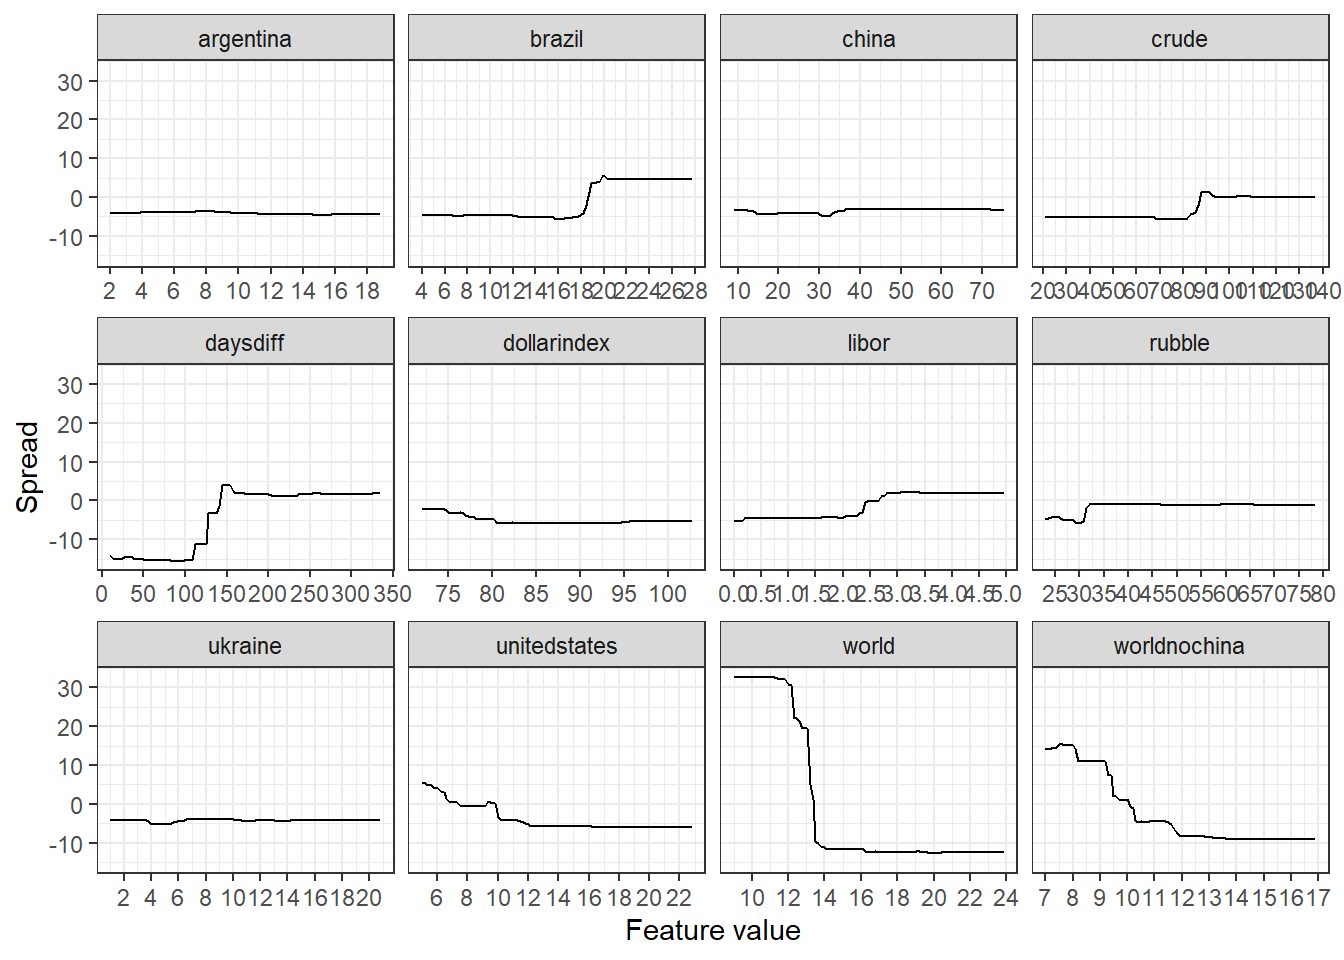
\includegraphics{calendar-spreads-macro-data_files/figure-latex/zz_critical_plot-1.pdf}

From the above we can clearly see some elbows in the line plots, these are ranges of the specific features where we can expect to see to big changes in the values of the spreads. The \emph{daysdiff} as an example, here we see a big decrease in the value of the spread when the feature value decreases below 150. It is interesting to note that at around 150 days before expiry of the front contract we are in the United States summer. This is the critical period for the corn market, if there is inclement weather here it will destroy the crop. However, most of the time after the weather stress period has passed the spread tends to collapse into a stronger contango. Other interesting critical values are found for single figure United States stock-to-usage numbers as well as global stock-to-usage numbers under 14\%. In both of these cases we should see big backwaration moves.

  \bibliography{book.bib,packages.bib}

\end{document}
